Les travaux de \cite{einstein} ont discuté beaucoup de choses. 

Une documentation complète sur l'usage de \LaTeX\ est accessible à partir des références \cite{latexcompanion, Knuth1984}.

Une image exemple d'une calculatrice scientifique est donnée par la figure~\ref{fig:MyFig}.

\begin{figure}[tbh]
	\centering
	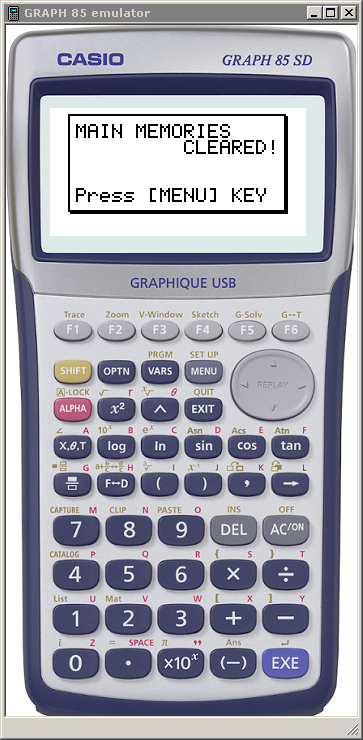
\includegraphics[width=4.25cm, height=7cm]{Casio}
	\caption{Exemple d'une calculatrice scientifque.}
	\label{fig:MyFig}
\end{figure}

La table~\ref{tab:MonTableau} montre un exemple.

\begin{table}
\centering
\caption{Mon tableau.}
\label{tab:MonTableau}
 \begin{tabular}{|l|c|r|}
	\hline
	A & 1 & \begin{tabular}{cc}
		a & b \\
		\hline
		c & d \\
	\end{tabular}
	\\
	B & 2 & \\
	C & 3 & \\
	D & 4 & \begin{tabular}{c}
		\hline
		x \\
		y \\
		z \\
		\hline
	\end{tabular}
	\\
	\hline
\end{tabular}
\end{table}

\cite{RICHARD20031667}

\textbf{AAAAAAAA}\textit{AAAAAAAAA}\underline{AAAAAAAAAAA}\textcolor{blue}{AAAAAA}AAAAAAAA
